\chapter{The Stern-Gerlach Experiment}

\section{Spin Angular Momentum}

Let's start with something that is pretty much as far away from the quantum world as possible -- the Earth and Sun.  With its total motion, the Earth has two kinds of angular momentum:  \emph{orbital} angular momentum $\vec{L}$ from its orbit around the sun, and \emph{spin} angular momentum $\vec{S}$, resulting from its 24 hour rotation.  Of course, the spin angular momentum in this case is due to adding up the orbital angular momentum $\vec{L}_i = \vec{r}_i \times \vec{p}_i$ of each of the tiny pieces of the Earth, but we'll keep the distinction -- it'll turn out that this is \emph{not} the case in quantum systems.\footnote{Note that the two kinds of angular momentum for the Earth point in different directions since the rotation axis of the Earth is tilted 23$^\circ$ from the orbital plane.}

The quantum version of this kind of system could be an electron in orbit around a proton -- a hydrogen atom.  The electron has orbital angular momentum just like the Earth (depending on what state it's in), and it also has spin angular momentum.  Careful, though, as the electron doesn't rotate like the Earth -- how can it when it has essentially no size or diameter to spin?  Despite this, it has measurable intrinsic angular momentum, which we'll call \emph{spin} $\vec{S}$.  Since spin is a vector, it has components $(S_x, S_y, S_z)$, and thus to specify the spin of the electron we need to use three different numbers; keep this in mind for later.

I'd like to explore this idea of spin without the complication of orbital angular momenmtum, so let's put a stationary electron all by itself in a magnetic field $\vec{B}$.  Since the electron isn't moving, the Lorentz force
\[
\vec{F} = q\vec{v} \times \vec{B}
\]
is zero.  But the electron's spin angular momentum gives it a magnetic dipole moment $\vec{\mu}$, and it's then possible for an \emph{inhomogeneous} magnetic field to exert a force given by (see Griffiths \emph{Introduction to Electrodynamics}, fifth edition, section 6.1.2)
\begin{equation}
\vec{F} = \grad (\vec{\mu} \cdot \vec{B}).
\label{eq_force_inhomo}
\end{equation}

\begin{figure}
\centering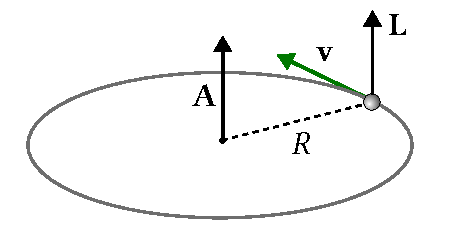
\includegraphics[width=0.5\linewidth]{Figures/Chapter 1/fig_circular_orbit.pdf}
\caption{A charged particle in a circular orbit has a magnetic dipole moment.}
\label{fig_circular_orbit}
\end{figure}

Now, we can calculate the magnetic dipole moment due to orbital angular momentum easily enough (we'll handle spin in a moment); Figure \ref{fig_circular_orbit} shows a particle in a circular orbit of radius $R$ and circular velocity $\vec{v}$.  If we think of this as a current loop, the dipole moment is just the current $I$ times the area $\vec{A}$,
\[
\vec{\mu} = I\vec{A}.
\]
The magnitude of the area vector is just $A = \pi R^2$ and the direction is perpendicular to the orbit, while the current will be the charge divided by the time it takes for the charge to make the orbit:
\[
I = \frac{q}{T} = \frac{q}{2\pi R / v}.
\]
The dipole moment is then
\[
\vec{\mu} = \left( \frac{1}{2} qvR, \text{ perpendicular to the orbit} \right).
\]
It's more useful, though, to put this in terms of the angular momentum $\vec{L} = \vec{r} \times \vec{p}$, which for a circular orbit is
\[
\vec{L} = \left( rmv, \text{ perpendicular to the orbit} \right).
\]
Finally, then, the magnetic dipole moment arising from orbital angular momentum is 
\begin{equation}
\vec{\mu} = \frac{q}{2m} \vec{L}.
\end{equation}

What changes for spin angular momentum?  It turns out to be only slightly different, and we can write
\begin{equation}
\vec{\mu} = \frac{gq}{2m} \vec{S},
\end{equation}
where $g$ is called the gyroscopic ratio or often just ``$g$-factor'' and, for an electron, is \emph{almost} $g = 2$.\footnote{We don't need to worry about this here, but each charged particle with spin has its own $g$-factor -- the proton has $g = 5.58$, for example.  These can be measuring and in some cases calculated theoretically, but it requires quantum field theory to do it properly.}

Let's go back to our electron in an inhomogeneous field. Take the field to be constant in the $x$ and $y$ directions but \emph{not} in the $z$ direction.  Then
\[
\vec{\mu} \cdot \vec{B} = \mu_x B_x + \mu_y B_y + \mu_z B_z,
\]  
and since the first two terms are constant, equation (\ref{eq_force_inhomo}) gives
\begin{equation}
\vec{F} = \grad ( \mu_z B_z ) = \mu_z \dfdx{B_z}{z} \, \hat{z} = \frac{gq}{2m} \dfdx{B_z}{z} S_z \, \hat{z}.
\label{eq_force_spin}
\end{equation}
The force on the electron in this case is directed along the $z$ direction and proportional to the component of spin angular momentum $S_z$ along that direction -- the more the spin aligns with the $z$ axis, the greater the force.
%
%
%

\section{The Stern-Gerlach Experiment}

In 1922 Otto Stern and Walther Gerlach used these ideas to measure the spin angular momentum of electrons.  Their experiment is shown in Figure \ref{fig_stern_gerlach_exp}, and they actually used silver atoms rather than electrons.  Why silver?  The atoms are electrically neutral, so there won't be any direct magnetic force on the atoms from the magnetic field, and the electronic configuration of silver is $1s^22s^22p^63s^23p^64s^23d^{10}4p^64d^{10}5s^1$.  Except for the outermost electron, all others are in closed shells, meaning we can ignore their contribution to the angular momentum of the silver atom.  The outermost electron is in an $s$-orbit, which has no orbital angular momentum -- so the only angular momentum of the entire silver atom is due to the spin of that one outer electron.

\begin{figure}
\centering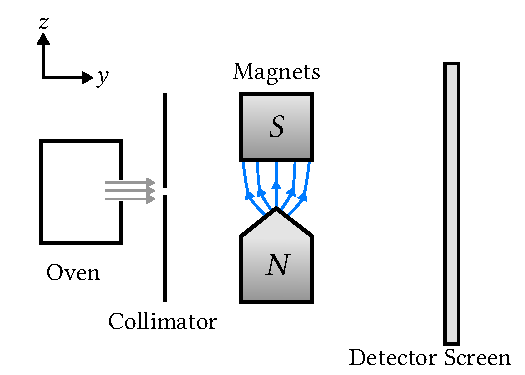
\includegraphics[width=0.6\linewidth]{Figures/Chapter 1/fig_stern_gerlach_exp.pdf}
\caption{The Stern-Gerlach experiments, in which silver atoms are deflected by an inhomogeneous magnetic field.}
\label{fig_stern_gerlach_exp}
\end{figure}

The Stern-Gerlach experiment proceeds as follows.  First, the oven boils silver atoms off of a solid piece of silver; the atoms are ``thermalized,'' meaning they come out in all directions and with random spin orientations.  A collimating slit produces a narrow beam of these atoms which pass between the magnets.  The magnets are constructed to create an inhomogeneous magnetic field, with the inhomogeneity in the $z$ direction; note that as shown the magnetic field gets stronger in the negative $z$ direction, so $\partial B_z / \partial z$ is negative in equation (\ref{eq_force_spin}).  Because the charge on the electron is negative as well, the force on a silver atom passing through the field will be up along $z$ if the spin has a positive $z$ component, and down along $-z$ if the spin has a negative $z$ component.  Finally, the deflection of each atom is measured when they hit the detecting screen.

What do we expect?  Well, as mentioned above, the oven thermalizes the atoms so the spin of the outer electron is in random directions.  That means the force on each atom will be random as well -- some atoms will get pushed up, some will get pushed down, and each with varying strength (up to some maximum for those spins that are entirely along $z$ or $-z$).  This expected result is shown in Figure \ref{fig_stern_gerlach_result_expected} (a).

\begin{figure}
\centering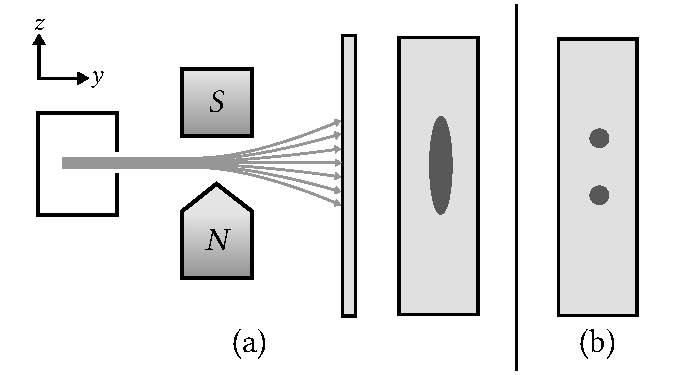
\includegraphics[width=0.8\linewidth]{Figures/Chapter 1/fig_stern_gerlach_result_expected.pdf}
\caption{(a) Classically expected result.  (b) Actual result showing quantization of spin angular momentum.}
\label{fig_stern_gerlach_result_expected}
\end{figure}

But that's not at all what Stern and Gerlach saw; instead, as Figure \ref{fig_stern_gerlach_result_expected} (b) shows, they detected only two locations where silver atoms hit the screen, corresponding to spin angular momentum values of either 
\[
S_z = +\frac{\hbar}{2} \quad \text{or} \quad S_z = -\frac{\hbar}{2}.
\]
This is clear evidence of the \emph{quantization} of angular momentum, something Niels Bohr suggested in 1913 when developing his model of the atom.  Evidently, every silver atom boiled off with the outermost electron having only two values for $S_z$.  Of course, this says nothing about the values of $S_x$ or $S_y$, or even the magnitude of the spin $S$.  And, actually, it turns out we can't even say they had these values of $S_z$ when they were created -- we can only say we measured $S_z$ to be either one or the other; more on this later.

%
%
%

\section{Extending the Experiments}

Before we discuss this further, though, I want to introduce some notation:
\begin{equation}
\label{eq_ket_definition}
\boxed{
\ket{\psi} \rightarrow \text{ Represents the state of a quantum mechanical system.}
}
\end{equation}
This notation is often called a ``ket,'' for reasons we'll see later, and it includes all possible information you could know about a particular quantum system.  Consider, for example, a silver atom that has been measured to have $S_z = +\hbar/2$.  We could represent the state of the atom by 
\[
\ket{+} \rightarrow \text{ State for which $S_z = +\hbar/2$ has been measured},
\]
although it's also common to use $\ket{\uparrow}$ or $\ket{+z}$.  This state is usually called ``spin up.''  Similarly, the ``spin down'' state is represented by 
\[
\ket{-} \rightarrow \text{ State for which $S_z = -\hbar/2$ has been measured},
\]
or  $\ket{\downarrow}$ or $\ket{-z}$.  Any particle that, when measuring a component of its spin angular momentum, has only two possibilities for the results is called a \emph{spin-1/2} particle; electrons, protons, and neutrons are all spin-1/2 particles.

Let's run through a few extensions to the original Stern-Gerlach experiment.  I've simplified the diagram of the original experiment in Figure \ref{fig_sg_0} to highlight the important steps: a beam of spin-1/2 particles (whether silver atoms or something else) is created, all in state $\ket{\psi}$, and sent to a Stern-Gerlach device (the magnets) to have the spin of each particle measured. In the case of the original Stern-Gerlach experiment, if a beam of 100 atoms were created, half of the atoms would be measured as spin up and half would be spin down.

Actually, we should be more careful -- we can't predict which atoms will be spin up and which will be spin down, and the process is inherently \emph{random}.  That means that we might get 49 spin up and 51 spin down, or 43 and 57, but if we increase the number of particles in the beam, we'll get closer and closer to exactly 50\% for each.   

\begin{figure}
\centering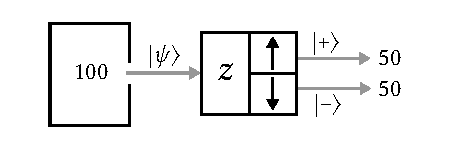
\includegraphics[width=0.6\linewidth]{Figures/Chapter 1/fig_sg_0.pdf}
\caption{A simplified diagram of the original Stern-Gerlach experiment.}
\label{fig_sg_0}
\end{figure}

In these experiments, we can think of the Stern-Gerlach device as an \emph{analyzer} -- it measures something.  But we can also think of it as a device for preparing a beam of particles all in the same known state; for example, each particle coming out of the top of the Stern-Gerlach device is in state $\ket{+}$, and we can use this knowledge to do further measurements. 

\subsection{Experiment 1}

It may be a basic question, but it's worth asking: once the particles are in state $\ket{+}$, for example, do they \emph{stay} in that state?  In Experiment 1 we'll test this by connecting another Stern-Gerlach device as shown in Figure \ref{fig_sg_1}, and sure enough all particles that enter the second analyzer come out with the same $\ket{+}$ state, and none become spin down.

That's a good thing: it means we can do repeated measurements and expect the same results.  Science would be tricky to do if things were otherwise.  But we should be a little careful, as quantum systems do evolve in time -- we'll learn about this later when we cover the Schr\"odinger equation -- so the repeated measurement should be made right after the first.

What if we moved the second device to accept the spin down particles from the first?  As you probably would guess, those particles would all be measured as being spin down, with no spin up particles at all.

\begin{figure}
\centering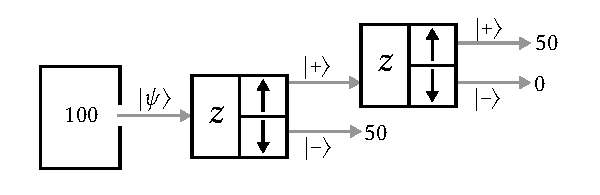
\includegraphics[width=0.8\linewidth]{Figures/Chapter 1/fig_sg_1.pdf}
\caption{Experiment 1: the spin up particles are sent to a second analyzer, where they're found to still be spin up. }
\label{fig_sg_1}
\end{figure}

\subsection{Experiment 2}

Now, we've been aligning the magnets in the Stern-Gerlach device so that the inhomogeneity in the magnetic field is along the $z$ axis, but we could have just as easily rotated it (or changed our axes) so that it is in fact along the $x$ direction.  Does anything change?  Well, no -- the coordinate system is just our choice and can't affect the actual physics that's happening, so we could just replace every $z$ in the discussion above with an $x$ with no other change.  But let's try something a little more interesting and combine a Stern-Gerlach device oriented along $z$ with one oriented along $x$; this is shown in Figure \ref{fig_sg_2}.

First, note the new notation; a particle in the state $\ket{+}_x$ has had its component of spin angular momentum along the $x$ direction measured to be $S_x = +\hbar/2$.  This is a different state that our previous spin up state (you might call it ``spin up along $x$'' or something similar) and requires new notation.  Note that I didn't bother with the $z$ subscript for our $S_z$ states; by convention, a ket without a subscript indicating direction will be along $z$.

\begin{figure}
\centering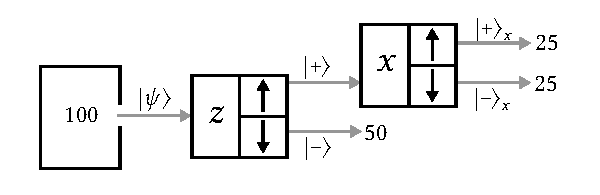
\includegraphics[width=0.8\linewidth]{Figures/Chapter 1/fig_sg_2.pdf}
\caption{Experiment 2: the spin up particles are sent to a second analyzer that has been rotated so that it measures $S_x$. }
\label{fig_sg_2}
\end{figure}

The results are different this time, with half of the spin up particles sent into the second Stern-Gerlach device being spin up along $x$ (so in state $\ket{+}_x$) and half being spin down along $x$ (in state $\ket{-}_x$).

Remember what we're measuring here:  the oven creates particles with a random spin orientation, and we measure half of those particles to have $S_z = +\hbar/2$, and then half of \emph{those} particles to have $S_x = +\hbar/2$.  We're missing the component of spin along the $y$ direction, so you might think we just add a third device to measure $S_y$ -- and then we'd know all three components of spin and therefore the vector $\vec{S}$.  But there's an interesting twist to this simple story that the next experiment will highlight.

\subsection{Experiment 3}

So, in Experiment 2, spin up (along $z$) particles have their spin along $x$ measured, and half are found to be spin up along $x$.  In Experiment 3, we take those particles that are spin up along both directions and send them into a third analyzer, this one oriented along $z$ as shown in Figure \ref{fig_sg_3}.  Just so that we're clear:  none of the particles sent into this last analyzer were measured to have $S_z = -\hbar/2$.  Despite this, half the particles analyzed by the last Stern-Gerlach device are found to be in state $\ket{-}$ along $z$.

What do we to make of these experimental results?  Evidently measuring $S_x$ has \emph{changed} the state of the particles; although they \emph{were} in state $\ket{+}$, after the measurement of $S_x$ they aren't any more.  

Some more terminology:  we call quantities that we can measure \emph{observables}, and we say that $S_z$ and $S_x$ are \emph{incompatible observables} -- measuring one affects our knowledge of the other.  Two other more famous incompatible observables are position and momentum from Heisenberg's uncertainty principle, although not all observables are incompatible -- you could know a particle's position and spin $S_z$ at the same time, for example.  

Obviously we could have used $S_y$ instead with no change to the results, so we run into a big problem measuring angular momentum:  we need three components to specify it, but can never know more than one at a time!  Actually, it turns out we can also know the \emph{magnitude} $S$ (we'll see why later), so at most we can specify the length and one component of the angular momentum vector.

\begin{figure}
\centering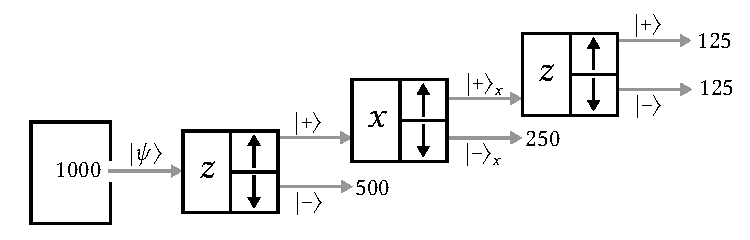
\includegraphics[width=\linewidth]{Figures/Chapter 1/fig_sg_3.pdf}
\caption{Experiment 3: the spin up particles are sent to a second analyzer that has been rotated so that it measures $S_x$, and then the particles in state $\ket{+}_x$ are sent to a third analyzer to have their spin component $S_z$ measured again. }
\label{fig_sg_3}
\end{figure}


\subsection{Experiment 4}

For this last experiment, we need to make some changes to the Stern-Gerlach device measuring $S_x$.  The details aren't too important as to how, but rather than measuring the spin $S_x$ observable, we'll recombine the two beams -- one pushed up by the magnetic field and one pushed down -- and send that combined beam into the last Stern-Gerlach device aligned along the $z$ direction.  But now the results are different, and we find that every particle is spin up along $z$.  It seems as though the middle device no longer has an effect on the initial $\ket{+}$ state of the particle; apparently it's the act of \emph{measurement itself} that alters the state, not the push by the magnetic field.  This is similar to the famous results from the double slit experiment -- measuring which slit the particle goes through destroys the interference pattern.

\begin{figure}
\centering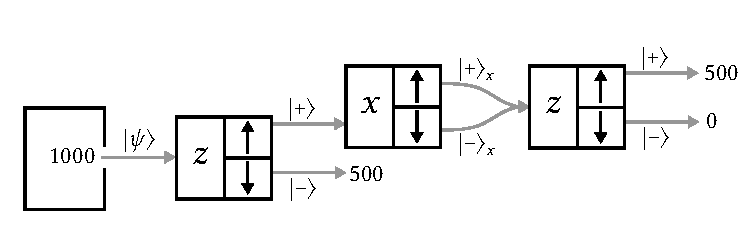
\includegraphics[width=\linewidth]{Figures/Chapter 1/fig_sg_4.pdf}
\caption{Experiment 4: We'll recombine the outputs from the $S_x$ device without measuring anything and send that combined beam into an $S_z$ device. }
\label{fig_sg_4}
\end{figure}


%
%
%


\section*{Problems}
\addcontentsline{toc}{section}{Problems}
\markright{Problems}%

\begin{problem}[Electron spin]
This whole chapter is about electron spin, but of course the electron doesn't really spin around like a top.  But let's pretend for a moment that an electron really is a tiny sphere, of radius
\[
r_e = \frac{e^2}{4\pi \epsilon_0 mc^2}
\]
(the so-called classical electron radius), and that it spins around its axis with angular momentum $S_z = \hbar/2$.  How fast would a point on the ``equator'' be moving?  Does this model make sense? 
\end{problem}

